\documentclass[12pt]{article}

\usepackage[utf8]{inputenc}
\usepackage[x11names,dvipsnames,svgnames,table]{xcolor}

% general incantations
\usepackage{indentfirst}
\usepackage[export]{adjustbox}
\usepackage{afterpage}
% \usepackage[british]{isodate}
\usepackage{graphicx}
\usepackage{placeins}
\usepackage{pdfpages}
\usepackage{algorithm2e}
\usepackage{array}
\usepackage[nottoc]{tocbibind}
\usepackage{booktabs}
\usepackage[most]{tcolorbox}
\usepackage{calligra}
\usepackage{caption}
\usepackage{datetime}
\usepackage{dblfnote}
\usepackage{dirtytalk}
\usepackage{dsfont}
\usepackage{fancyhdr}
\usepackage{fix-cm}
\usepackage[T1]{fontenc}
\usepackage{textcomp,gensymb} %for \degree C symbol
\usepackage{graphicx}
\usepackage{lipsum}
\usepackage{listings}
\usepackage{transparent}
\usepackage[everyline=true,framemethod=tikz]{mdframed}
\usepackage{mparhack}
\usepackage{multicol}
\usepackage{multirow}
\usepackage{parskip}
\usepackage{lscape}
\usepackage{pdflscape}
\usepackage{pdfpages}
\usepackage{placeins}
\usepackage{rotating}
\usepackage{setspace}
\usepackage{subcaption}
\usepackage{threeparttable}
\usepackage[normalem]{ulem}
\usepackage{verbatim}
\usepackage{soul} %highlighting, strike through etc.

%Automated appendices
\usepackage[titletoc,title,header]{appendix} %advanced functionality

%language settings
\usepackage[utf8]{inputenc}

%page setup
%this where we adjust the binding offset, if relevant
\usepackage[a4paper]{geometry}
\usepackage{lastpage} % for page 1 of n footers

%cross referencing
\usepackage[hidelinks]{hyperref}
\usepackage{cleveref}

%maths stuff
\usepackage{amsmath}
\usepackage{mathtools}

\setcounter{secnumdepth}{5}

%lists
\usepackage{enumitem}



\definecolor{codegreen}{rgb}{0,0.6,0}
\definecolor{codegray}{rgb}{0.5,0.5,0.5}
\definecolor{codepurple}{rgb}{0.58,0,0.82}

\lstdefinestyle{mystyle}{
    commentstyle=\color{codegreen},
    keywordstyle=\color{magenta},
    numberstyle=\tiny\color{codegray},
    stringstyle=\color{codepurple},
    basicstyle=\ttfamily\footnotesize,
    breakatwhitespace=false,         
    breaklines=true,                 
    captionpos=b,                    
    keepspaces=true,                 
    numbers=left,                    
    numbersep=5pt,                  
    showspaces=false,                
    showstringspaces=false,
    showtabs=false,                  
    tabsize=2
}

\lstset{style=mystyle}

%line spacing
\linespread{1.5}
\setlength{\parindent}{5ex}

\begin{document}

\pagenumbering{Roman}
\begin{titlepage}
    \thispagestyle{empty}
    \setlength\headheight{0pt} 
    \begin{center}

    \begin{center}
    
\includegraphics[width=0.65\linewidth]{images/ucc_logo.png}            
    \end{center}	

        \vspace{0.25cm}
        \vspace{0.25cm}
        {\scshape\Large Final-Year Project Report \\ BSc in Computer Science\par}
        \vspace{0.5cm}

        {\Large\bfseries Python Package for Enumerating Combinatorial Objects\par}
        
        \vspace{0.5cm}
        {\Large\itshape Donnchadh Durkan\par}
        Department of Computer Science
        \vspace{0.25cm}

    \vspace{1cm}
    Supervised by\par
    Dr Kieran T. Herley \\
    Department of Computer Science\par
    \vspace{1.5cm}
    \large
    April 2020

    \end{center}
\end{titlepage}

\section*{Abstract}
\topskip0pt
\vspace*{7em}
The goal of the project is to create a programmer-friendly Python package
that allows developers to access useful combinatorial algorithms. The package aims to build on the
foundations of Donald Knuth’s work in his book The Art of Computer Programming Volume 4A:
Combinatorial Algorithms, and provides efficient implementations of several of the algorithms
discussed there.

Specifically, the package will include the ability to generate all permutations and combinations of a
sequence, generate all trees for a given number of vertices, generate all partitions for a given
integer, and all partitions for a given set. In addition to this functionality, the package will also allow for the random generation of a mapping of the objects mentioned. The algorithms will be tested
against implementations provided by existing Python packages, such as itertools, which will provide
a useful benchmark for their efficiencies, and give expectations for how the algorithms should
function in terms of inputs and outputs.
\\\\
Keywords: Combinatorics, permutations, combinations, partitions, trees.
\vspace*{\fill}
\pagebreak

\section*{Declaration of Originality}
\topskip0pt
\vspace*{7em}
In signing this declaration, you are conforming, in writing, that the submitted work is entirely your own original work, except where clearly attributed otherwise, and that it has not been submitted partly or wholly for any other educational award.

I hereby declare that:
\begin{itemize}
    \item this is all my own work, unless clearly indicated otherwise, with full
and proper accreditation;
    \item with respect to my own work: none of it has been submitted at any educational institution contributing in any way to an educational award;
    \item with respect to another’s work: all text, diagrams, code, or ideas,
    whether verbatim, paraphrased or otherwise modified or adapted, have
    been duly attributed to the source in a scholarly manner, whether
    from books, papers, lecture notes or any other student’s work, whether
    published or unpublished, electronically or in print.
\end{itemize}

Signed: Donnchadh Durkan 
\includegraphics[width=0.5\linewidth]{images/signature.PNG}

Date: \today
\vspace*{\fill}
\pagebreak

\section*{Acknowledgements}
\vspace*{7em}
I wish to express sincerest thanks to Dr Kieran T. Herley for his valuable and constructive feedback throughout the project. His unwavering dedication to provide assistance has been greatly appreciated. 

I would also like to thank David Fox and Tim Lehane for their continued friendship. They have been a tremendous source of positivity and happiness.

Finally, I wish to thank my parents, as well as my partner, for their support and encouragement.
\vspace*{\fill}
\pagebreak

\tableofcontents

\cleardoublepage
\pagenumbering{arabic}


% INTRODUCTION -------------------------------------------------------------------------------------------
\section{Introduction}

\subsection{Overview of Combinatorics}
Combinatorics describe the different patterns a finite set or structure can be arranged into. These patterns are often referred to as combinatorial objects. A combinatorial object is an object which has a one-to-one, or injective, mapping to a finite set of integers. Some examples include permutations, combinations and partitions of sequences. 

The ability to generate these objects is useful in a variety of areas. Algorithm design and analysis relies on the ability to generate test data from combinatorial objects. This allows the calculation of average and worst-case complexity, which can drive the improvement of the algorithms. Alternatively, some problem spaces are too large to rely on deterministic algorithms, as they lead to unrealistic run-times. A solution to this is to use randomized or approximation algorithms, which aim to reduce the problem space. These algorithms lean heavily on combinatorial methods for analysis.

\subsection{Project Aims}
The goal of the project is to create a programmer-friendly Python package that allows developers to access useful combinatorial algorithms. The package primarily aims to build on the foundations of Donald Knuth’s work in his book \textit{The Art of Computer Programming Volume 4A: Combinatorial Algorithms}, and provides efficient implementations of several of the algorithms discussed there. Specifically, the package will include the ability to generate all permutations and combinations of a sequence, generate all trees for a given number of vertices, generate all partitions for a given integer, and all partitions for a given set. In addition to this functionality, the package will also allow for the random generation of a mapping of the objects mentioned.

\textit{Itertools} is an existing Python package which provides permutation and combination algorithms that mirror certain aspects of the functionality required \cite{itertools}. As a result, \textit{itertools} will serve as a useful benchmark for the new package. All new algorithms should be tested against it, and should provide at least the same functionality. This package aims to extend beyond \textit{itertools'} capabilities, and should encourage linked functionality between the different combinatorial areas of interest.

\subsection{Deliverables}
The project was achieved by approaching the task one combinatorial object at a time. In the case of permutations and combinations, Knuth provided numerous algorithms which all served the same purpose. Therefore careful study of his writings and analysis was needed in order to reduce the number of algorithms as potential candidates for the package. 

Once these algorithms were selected, they were implemented in Python and rigorously test and compared against each other. It is rare that one algorithm outperforms all others in every scenario, therefore it was imperative that the algorithms were considered on several different merits. 

The end result of the project is a package which proudly offers effective and efficient implementations of Knuth's algorithms, as outlined previously. Despite the utilization of C in \textit{itertools}, which will be discussed later, this package boasts competitive algorithms for generating permutations and combinations.
\pagebreak

% ANALYSIS -----------------------------------------------------------------------------------------------
\section{Analysis}
\subsection{Combinatorial Objects}
To fully understand the aims and capabilities of the package, it is important to have an insight into different combinatorial objects. There are four main objects covered by Knuth that the package aims to have implementations for.

\subsubsection{Permutations}
A permutation is an arrangement of a finite number of items in a set. Subsequently the order that the items appear in is the defining aspect of a permutation. Permutations are generated by altering this order. Take the set \{A,B,C\}, where \(n=3\). All possible permutations of size \(k=3\) of this set are:\\
(A,B,C), (A,C,B), (B,A,C), (B,C,A), (C,A,B), (C,B,A)

This package predominantly deals with the case where \(n=k\). Consequently, the calculation for the number of permutations of size \(n\) is trivial. As the order matters, there are \(n\) options for the first item, \(n-1\) for the second item and so on, down until there is only one option for the final item. Putting this together gives:
\[n(n-1)(n-2)...(1) = n!\]

However, when \(n \neq k\), the factorial process must be stopped after multiplying \(n-k\) terms. Mathematically, the simplest way to achieve this is to divide by \((n-k)!\), leaving the formula:
\[\frac{n!}{(n-k)!}\]

Factorial functions grow at a faster rate than exponential functions, with the exception of the superexponential \(n^n\). While the example above only has six permutations, increasing \(n\) from \(n=3\) to \(n=10\), increases the number of permutations to 3,628,800.

This rapid growth ensures that any algorithms in this package must provide intuitive ways to interact with the permutations.

\subsubsection{Combinations}
Combinations are not dissimilar to permutations, with the exception being that order of the elements in the set does not matter. Often, there is a desire to know how many subsets of size k can be taken from a set of size n.

Again, take the set {A,B,C} with \(n=3\) and \(k=3\). Therefore, there is only 1 possible combination:\\
(A,B,C)

However, for the same set, but \(k=2\), we get 3 combinations:\\
(A,B), (A,C), (B,C)

The number of combinations is calculated building off of the formula for the number of permutations, which works out as: 
\[\frac{n!}{k!(n-k)!}\]

\subsubsection{Partitions}
There are two type of partitions, integer partitions and set partitions. In the case of the former, the process is characterized taking a positive integer \(n\), and breaking it up in the sum of positive integers. For \(n=3\), the partitions are: \\
(\(3\)), (\(2+1\)), (\(1+1+1\))

A major use case for integer partitions are algorithms that calculate the amount of change required to give a customer upon payment. By constraining the integers that can appear in the partition to represent monetary values, a greedy approach can be taken to arrive quickly at the optimal solution, that is, the least amount of notes and coins required.

Set partitions refer to the division of a set into subsets. A partition of a set assigns each element in the set to exactly one subset. The subsets are non-empty, they must contain at least 1 element. The amount of subsets that exist is based on the number of partitions. 1 partition means 2 subsets, 2 partitions means 3 subsets, and so on. It is crucial to note that subsets are not necessarily proper subsets, \{\{1,2,3\}\} is a valid partition of \{1,2,3\}.

\subsubsection{Trees \& Forests}
Trees and forests are similar structures, they are vertex-edge graphs. Any vertex can have at most one parent, but can have multiple children. The primary difference between the two structures is that there is exactly one path between any 2 vertices in a tree, however there may not be a path between any two vertices in a forest. In this context, forests are acyclic, and both trees and forests are undirected.

Structures like these have many uses, such as storing hierarchical data. They are dynamic, meaning it is simple to add and remove vertices from them as needed. Due to their non-linear shape, it is harder to generate all trees or forests. This is reflected in the design and implementation of the algorithms, which will be discussed later on.

\subsection{Shaping the Package}
In order to decide the specific functionality of the package, careful analysis of existing material as well as \textit{itertools} needed to be completed. The investigation began by looking at \textit{The Art of Computer Programming Volume 4A: Combinatorial Algorithms}. Permutations were explored first, and it became apparent that an adequate algorithm for generating uniformly random permutations was not mentioned in the book. Further research in this area led to an algorithm popularized by Knuth, known as \textit{Knuth Shuffles} \cite{knuth_shuffle}, but in spite of its name, it was originally designed in 1938 by Fisher \& Yates \cite{rand_perm}.

Combinations is the only area of the project where the package does not match up to \textit{itertools} capabilities. Knuth usually examines combination generation algorithms where replacement of objects in the set does no occur. Subsequently this package does not provide the functionality for combination with replacement.

Much like permutations, Knuth does not write about algorithms for generating uniformly random combinations. Fortunately, Knuth does propose such an algorithm in \textit{The Art of Computer Programming Volume 2, Seminumerical Algorithms} \cite{rand_comb}.

Itertools only provides set partitioning through an unofficial extended toolset \cite{itertools_extension}. Adding Knuth’s work to the package is an extension beyond what is available in \textit{itertools}. Knuth provides algorithms for integer partitioning, set partitioning and multiset partitioning. A random set partition algorithm by Nijenhuis \& Herbert \cite{rand_set_part} completes the partition algorithms. With regards to tree generating algorithms, Knuth fully covers all aspects of this in the book, and as such there is no need for further research into this area.

Knuth does not scrutinize these algorithms' complexities. By implementing several algorithms for the tasks, it becomes easier to evaluate them against each other. 

\subsection{Python Implementation}
% How does python facilitate the implementation of the package
It is important to note that \textit{itertools} is a Python API for a C backend. Therefore, it is difficult to meaningfully compare \textit{itertools'} algorithms run times to a pure Python implementation, due to Python being an interpreted language as opposed to C which is compiled. \textit{Cython}, a static compiler for Python \cite{cython}, should be utilised in order to speed up run times by essentially stripping back some Pythonic features such as dynamic typing. The use of \textit{Cython} will not guarantee matching times with \textit{itertools}, but the intention is that it will provide competitive times.

While \textit{Cython} solves some issues, it creates others. \textit{Cython} does not support generator functions as part of \lstinline{cdef} functions. Immediately this limits the benefits that are achievable using \textit{Cython} if generators are required. Alternatively, rather than using generators, it may be possible to use \textit{numpy} arrays to store sequences. This would give enormous gains in runtime, but despite \textit{numpy} using less memory, that concern remains.

As explained in section 2.1.1, the number of objects being generated can quickly reach cumbersome levels. It is in feasible to create arrays containing millions of objects, and store them in memory. To counteract this issue, the package makes use of Python's \textit{generator} functions \cite{generator}. They are functions which return generator objects, allowing developers to generate the next item in a sequence only when called to do so.

The package attempts to maintain uniform usability throughout. Input sequences for the functions can take the form of any iterable object. This means that the generator object returned from any of the functions in the package can be used as an input for several of the other functions, achieving the linked functionality.

\pagebreak

% DESIGN -------------------------------------------------------------------------------------------------
\section{Design}

\subsection{Technologies}
For the most part, the package does not depend on any libraries outside of the default Python libraries. The exception to this being the \textit{random} library, as a source of entropy is required to generate uniformly random combinatorial objects.

As discussed previously, permutation and combination algorithms employ the use of the static compiler \textit{Cython} to improve the time taken to generate the next object in the sequence. The package aims to be as lightweight as possible, by avoiding all unnecessary overheads.

\subsection{Testing Generator Algorithms}
The initial method for testing the algorithms begins by simply reading Knuth's work. He often discusses algorithms which are not necessarily the most efficient, simply because they take a unique approach. Following this idea, it is possible to rule out several algorithms for this reason, or due to unnecessary requirements to use them. Algorithm G for generating permutations \cite{perm_G} is a good example of this, where a Sims table is required for the algorithm to work. This needless overhead is a hindrance to a developer in nearly all cases.

Once the remaining algorithms are chosen and implemented, it follows logically that they should be timed, given Knuth's evasion of complexities. The next question is how should the algorithms be timed, where there are two possible approaches.

\begin{enumerate}
  \item Use the generator functions to step through the algorithm one object at a time. Record the time it takes to generate the next object.
  \item Wrap the function call in Python's built in function \lstinline{list()}, which will automatically create a list containing all the objects that the generator will output. The total time taken from start to finish is recorded, and this is divided by the number of items in the list to get the mean time taken per object generation.
\end{enumerate}

Option two appears to be the better approach. The first option will lead to a large number of data points, which can be difficult to maintain when the input sequence is large. Furthermore, it is also possible that option is affected by outliers due to patterns in the sequences that may occur later on. As a result, option two will give a more accurate estimate of the mean time taken per object generated.

This value can then be compared against the values from the other algorithms, as well as those provided by \textit{itertools}, and the \textit{Cython}-refactored algorithms to determine which will return the best average use case.

\subsection{Testing Random Algorithms}

Despite formal proofs of randomness being given for the algorithms used in this package, there is no guarantee that the Python 'translations' maintain this property. Testing the randomness of algorithms can be challenging given that their outputs are inherently unpredictable, so unit testing is not the best method.

One method involves running these algorithms with a relatively small input sequence, for example a sequence of size four. The algorithms would run repeatedly for 100,000 iterations, where the frequency of the results would be tracked. An input sequence of size four is advantageous compared to a greater size, as it is more likely to lead to a better distribution of values, and there number of possible values is more manageable (\(4!=24\) possible permutations in this case). 100,000 iterations is chosen to ensure a good distribution of values also. It will also serve to highlight any significant anomalies in the actual frequencies. By graphing the actual frequencies against the expected frequencies, any major discrepancies would be clearly visible on graph. This would act like an informal examination of the results to determine randomness.

While the visual aid of the graph is useful, it is too vague to be able to draw any real conclusions. The chi-squared test is a hypothesis test which evaluates the relationship between expected and actual frequencies of a given category. This makes it an excellent candidate for assessing the Python algorithms randomness. By interpreting the \(p-value\) returned by the test, a clearer idea is given about the true randomness. Although this is not a formal proof, it should serve satisfactorily to verify the integrity of the algorithms.

\pagebreak

% IMPLEMENTATION -----------------------------------------------------------------------------------------
\section{Implementation}

\subsection{Software Implementations}
The structure of the algorithms remain simple at their core. They were implemented using as many of Python's native features as possible. This is because Python offers excellent built-in methods for objects like lists, which feature widely throughout the package. Efficient manipulation of lists is key in achieving optimal results.

Please note that some algorithms may have the same name, due to their appearance in different sections of the book.

\subsubsection{Permutations}
Four algorithms for generating permutations were chosen to be evaluated.
\begin{enumerate}

\item The first algorithm \cite{perm_L}, aptly named Algorithm L, visits the permutations in lexicographic order. Lexicographic order is advantageous as it essentially represents counting in a variable base. It is familiar to the user and is often one of the only approaches where you can predict the next sequence that will be generated.

\begin{figure}[h]
\centering
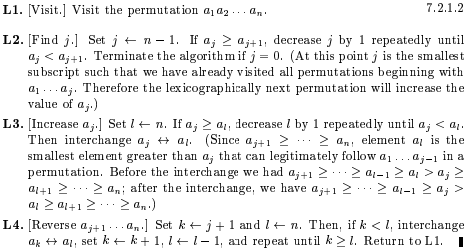
\includegraphics[width=0.8\textwidth]{images/perm_L.PNG}
\caption{Knuth's description of Algorithm L \cite{perm_L}}
\end{figure}

This algorithm has an interesting property, where the input sequence must be sorted. This is not a desirable feature, as sorting can be time-consuming and it can not deal with sequences containing duplicates.

To work around this issue, the algorithm creates a new array \lstinline{[0, 1, ..., n-1]} where n is the length of the input sequence. The algorithm then alters this array, rather than the original. By taking this approach, a sorted sequence is guaranteed containing no duplicated. This array acts as indices for the original. Using Python's list comprehension, the generator object can serve the sequences efficiently to the user.

\item Algorithm P, plain changes, only requires the input sequence to contain distinct elements. Again, a new array of indices is created to avoid this issue arising.

\begin{figure}[h]
\centering
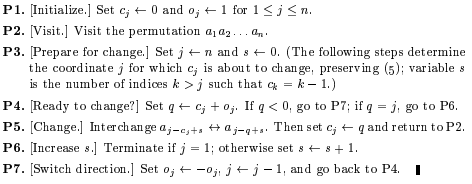
\includegraphics[width=0.8\textwidth]{images/perm_P.PNG}
\caption{Knuth's description of Algorithm P \cite{perm_P}}
\end{figure}

Plain changes works by maintaining a second array, describing the direction that the elements in the sequence can "move". An element is mobile if it is pointing in the direction of one of its neighbours, and it's value is greater than its neighbour's. Each iteration, the largest mobile gets to move, creating a new sequence.

\item Algorithm E is similar to Algorithm P. It uses two arrays to control the next element swap that takes place. 

\begin{figure}[h]
\centering
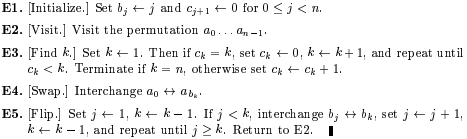
\includegraphics[width=0.8\textwidth]{images/perm_E.PNG}
\caption{Knuth's description of Algorithm E \cite{perm_E}}
\end{figure}

While Algorithm P only swapped elements that were adjacent, this always swaps the first element in the array to generate the next sequence. The additional control essentially constrains the swaps, which increases the efficiency of the algorithm.

\item The Fisher-Yates-Knuth Shuffle algorithm generates a random permutation of an input sequence \cite{rand_perm}\cite{knuth_shuffle}.

\begin{figure}[h]
\centering
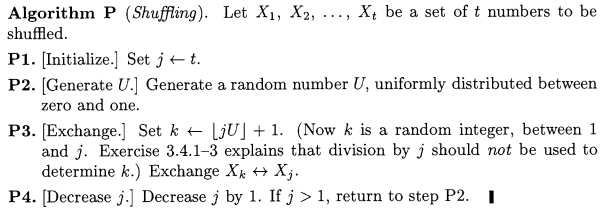
\includegraphics[width=0.8\textwidth]{images/rand_perm.PNG}
\caption{Description of Knuth Shuffles in \textit{Seminumerical Algorithms} \cite{knuth_shuffle}}
\end{figure}

The algorithm requires a source of entropy to ensure its randomness. In the Python implementation, \(k\) is generated directly using the \textit{random} library.

\end{enumerate}

\subsubsection{Combinations}

Four algorithms for generating combinations were chosen to be evaluated.

\begin{enumerate}
\item The first algorithm is the straightforward once again. It proposes to visit all combinations in lexicographic order.

\begin{figure}[h]
\centering
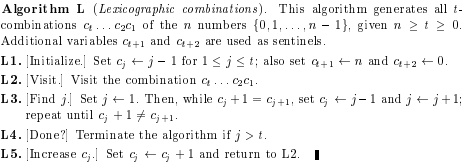
\includegraphics[width=0.8\textwidth]{images/comb_L.PNG}
\caption{Description of Algorithm L \cite{comb_L}}
\end{figure}

Algorithm L finds the rightmost value which can still be increased. Once it has found and increased this value, it then reorders all previous elements to make the smallest value possible.

The description of the algorithm specifies constraints on the sequence that forms the combinations. This does not inhibit the practicality of the algorithm, as these numbers can be used as indices in the same way they were used for generating permutations.

\pagebreak

\item Algorithm T is almost identical to Algorithm L. The difference occuring at stage T3. It identifies one of the most common situations that occurs when computing the next combination, and essentially hard-codes the best approach to take in that scenario.

\begin{figure}[h]
\centering
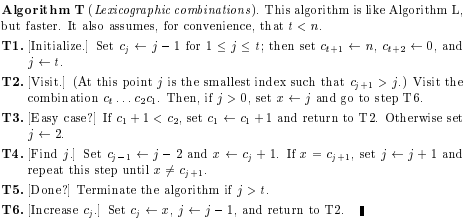
\includegraphics[width=0.8\textwidth]{images/comb_T.PNG}
\caption{Description of Algorithm T \cite{comb_T}}
\end{figure}

Any minor losses at runtime due to the additional \lstinline{if} statement are cancelled by the gains made when it returns \lstinline{True}.

\pagebreak

\item Algorithm C introduces the idea of near-perfect scheme \cite{comb_C}. They are characterized by the element in the sequence not having to move more than two indices away from it's current location to  compute the next combination.

\begin{figure}[h]
\centering
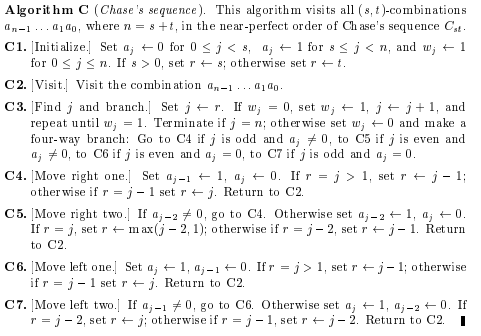
\includegraphics[width=0.8\textwidth]{images/comb_C.PNG}
\caption{Description of Algorithm C \cite{comb_C}}
\end{figure}

\pagebreak

\item Algorithm S employs a selection sampling technique for \(n \choose k\). This works well when \(k \leq n/2\).

\begin{figure}[h]
\centering
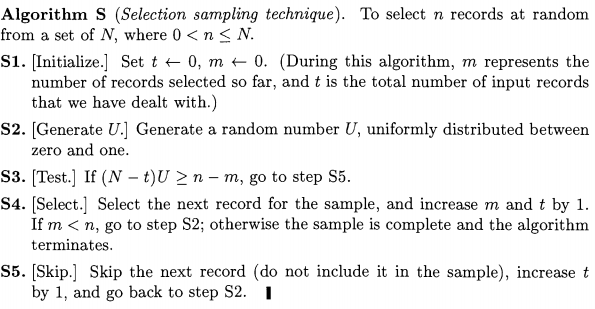
\includegraphics[width=0.8\textwidth]{images/rand_comb.PNG}
\caption{Algorithm S which generates a random combination \cite{rand_comb}}
\end{figure}


However, there are improvements that can be made in the case of \(k > n/2\). In this scenario, the problem turns from selection sampling to rejection sampling. The same process of selecting an element from the sequence takes place, but the element is then thrown away, rather than kept. 
\end{enumerate}


\pagebreak
\subsubsection{Partitions}
Knuth did not cover a wealth of algorithms for partitioning in general. Two algorithms for integer partitioning were implemented. 

\begin{enumerate}
\item The first algorithm generates all integer partitions for a given positive integer.

\begin{figure}[h]
\centering
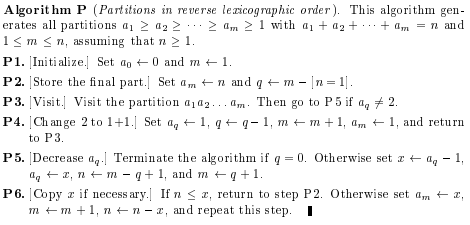
\includegraphics[width=0.8\textwidth]{images/int_part_P.PNG}
\caption{Algorithm P, for generating integer partitions \cite{int_part_P}}
\end{figure}

Knuth discusses the key to the algorithm, which lies in P4 \cite{int_part_P}. When a '2' is present in a partition, it is trivial to then find the following partition. The '2' is simply changed to a '1', and an additional '1' is appended to the end of the sequence.

\pagebreak


\item Algorithm H returns the integer partitions of a given size in colexicographic order.

\begin{figure}[h]
\centering
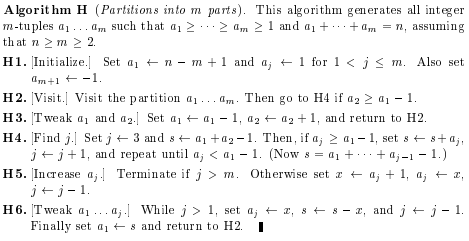
\includegraphics[width=0.8\textwidth]{images/int_part_H.PNG}
\caption{Algorithm H, for generating integer partitions of \(m\) parts \cite{int_part_H}}
\end{figure}

Despite Algorithm H being a niche case of Algorithm P, it may be worth investigating their performances when Algorithm H is called time and again in order to generate all possible integer partitions.

\end{enumerate}

Knuth provided one algorithm for set partitioning, and another for multiset partitioning. External research outside the scope of Knuth's work was undertaken so that the package had the capability of generating random set partitions.

\begin{enumerate}
\item By applying the previous idea of creating a new array representing indices, the decision was taken to only implement the algorithm for generating all set partitions. Using the indices would allow multisets to be passed in as arguments, and the algorithm would be able to handle it adequately.
    
\begin{figure}[h]
\centering
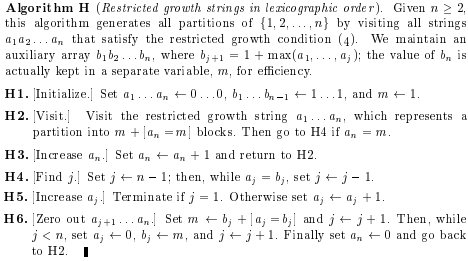
\includegraphics[width=0.8\textwidth]{images/set_part_H.PNG}
\caption{Algorithm H, for generating all set partitions of a sequence \cite{set_part_H}}
\end{figure}
    
\pagebreak
    
\item It is important to understand that this algorithm was designed for the \textit{Fortran} programming language, a verbose, low-level language. Python's strong list manipulation capabilities allow the algorithm to be implemented more smoothly with some minor adjustments. 

\begin{figure}[h]
\centering
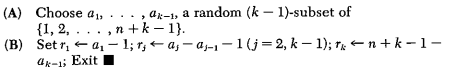
\includegraphics[width=0.8\textwidth]{images/rand_set_part.PNG}
\caption{Nijenhuis \& Herbert's algorithm for \(k\) random partitions of a set. \cite{rand_set_part}}
\end{figure}

\(r\) represents the array containing the \(n\) elements of the input set. The reason it has more than \(n\) elements is that it needs to be able to represent where the partitions occur as unique elements in the set. 

Due to list slicing in Python, there is no need to make a longer list, since they are mutable and the values can be easily changed. The first step remains the same; randomly choose where the partitions will occur. The implementation only differs in part 2, where the list is directly altered in Python to give an output which aligns with Algorithm H for set partitioning.

\end{enumerate}

\subsubsection{Trees}
Three algorithms were implemented in Python for tree generation. 

\begin{enumerate}
\item Algorithm P generates all trees of size \(n\), represented as nested parentheses.

\begin{figure}[h]
\centering
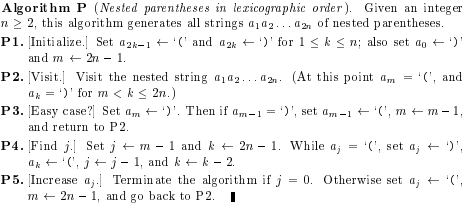
\includegraphics[width=0.8\textwidth]{images/tree_P.PNG}
\caption{Description of Algorithm P \cite{tree_P}}
\end{figure}

\item Algorithm B works specifically for binary trees. Rather than representing the structure using nested parentheses, the algorithm maintains two arrays which describe the left and right links between the nodes.

\begin{figure}[h]
\centering
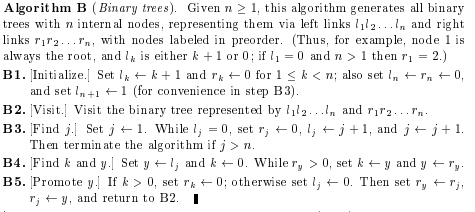
\includegraphics[width=0.8\textwidth]{images/tree_B.PNG}
\caption{Description of Algorithm B \cite{tree_B}}
\end{figure}

This representation creates some confusion as it is not as intuitive as the nested parentheses model. Furthermore, it also creates an issue of morphing it into a tree object.

\item Algorithm W offers the functionality of generating random trees of a given size. This algorithm returns trees as nested parentheses.

\begin{figure}[h]
\centering
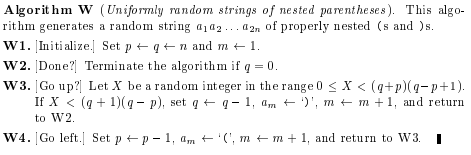
\includegraphics[width=0.8\textwidth]{images/tree_W.PNG}
\caption{Description of Algorithm W \cite{tree_W}}
\end{figure}

\end{enumerate}
\vspace{1cm}
\begin{figure}[h]
\centering
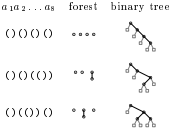
\includegraphics[width=0.4\textwidth]{images/table1.PNG}
\caption{A partial table showing the relationship of nested parentheses to trees and forests. \cite{tree_P}}
\end{figure}

It is interesting to note the representation of the trees as nested parentheses. They can represent both a tree, and a forest as seen in figure 16. Custom parsers for the parentheses allow these interpretations. In contrast to this, the array of integers produced by Algorithm B is not as straightforward to manage. Any benefits made in the specific nature of the algorithm are lost when translating the output to a graph.

\subsection{Experiments}
% software apparatus, methodology
\subsubsection{Testing Generator Algorithms}

The algorithms should be tested with varying lengths of input sequences. By calculating the mean time it takes to transform one valid combinatorial object to another, the expectation is that this value should remain similar regardless of the length of the input sequence.

The experiments are be carried out in Python using the \textit{timeit} library to generate accurate times, and the results are plotted using Excel and the \textit{matplotlib} Python library. In the cases of permutations and combinations, the basic Python algorithms will be tested against the \textit{Cython} attempts, as well as \textit{itertools'} capabilities.

It is important to acknowledge the shortcomings of time-based experiments when assessing algorithms. Any times found will be intrinsically linked to the hardware that the experiments are run on. However, since the goal is simply to find the 'quickest' algorithm to complete the task, this is still achievable since all algorithms will be gated by the same limitations.

\subsubsection{Testing Random Algorithms}
This project does not attempt to formally verify the randomness of its algorithms. They have already been proven, and as such, this randomness needs to be verified to ensure that this property was not lost in the Python implementations.

The \(p-value\) returned by the chi-squared test in this case represents the probability that the actual sequence of occurs, on the condition that expected frequencies are, in fact, uniformly distributed. The \(p-value\) returned is expected to be a relatively small value, given the number of possible partitions of 100,000 trials. Regardless, it should still be clear that the randomness of the algorithms is verified by this hypothesis test. 

\textit{SciPy} is a Python library which implements the chi-squared test \cite{chi_square}. Only one argument is required as input, the observed frequencies. It assumes a uniform distribution of the expected frequencies to create the null hypothesis. A double bar graph is presented to give a visual aid for the results.

\subsection{Incomplete Work}
% algorithm T for combinations doesn't work
\subsubsection{Combinations - Algorithm T}
Algorithm T for generating combinations \cite{comb_T} was not successfully implemented using Knuth's description. The current version of the algorithm in Python visits sequences in the wrong order, and duplicates values in the sequence erroneously. 

In it's current state, it is inadequate and does not serve its purpose. Its inclusion in the package is revoked, and no tests will be carried out the incorrect algorithm.

% add custom parsers for tree generation
\subsubsection{Tree Parsing}
In their current states, Algorithm P and Algorithm W return sequences of nested parentheses as mentioned above. Presently, the onus is on the user to decide the interpretation of this sequence, either as a binary tree or as a forest.

In future iterations of this package, it would be advantageous to have these functions take in an additional value, which would specify the return type of the sequences. The functionality for tree or forest parsing would come bundled with the package.

\pagebreak

% EVALUATION ---------------------------------------------------------------------------------------------
\section{Evaluation}
\subsection{Appraisal of Completed System}
The package meets the most expectations set out at the beginning. It contains methods that facilitate the generation of permutations, combinations, partitions and graphs. At its core, it is a developer-friendly package, with many obvious uses. The package acts as a centralized base for the most common combinatorial tasks.

Initially, the idea of graph theory was teased. Graph theory is an area of combinatorics which features widely across computer science, from networking to real-world maps. Unfortunately, due to time restrictions, graph theory had to be excluded from the scope of this project.

\subsection{Testing the Package}
Basic unit tests were setup to ensure that the algorithms provided the desired output for randomly selected input sequences. The amount of objects generated are tallied so that they match with the correct amount. By storing all the objects in a list, the list can be converted to a set, where any duplicates will be removed. Should the length of the list not equal the length of the set, it is clear that the algorithm is not functioning properly as it is outputting duplicated values.

\subsubsection{Permutations}
The three algorithms for generating all permutations of a sequence, mentioned in section 4.1.1, were timed using the \textit{timeit} library. The total time taken to generate all of the permutations can be seen in figure 17, where \(n\) represents the size of the input sequence.

\begin{figure}[h]
\centering
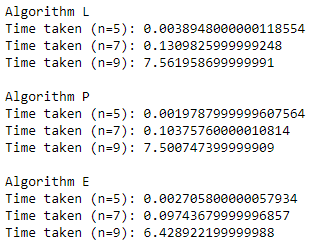
\includegraphics[width=0.5\textwidth]{images/perm_times.PNG}
\caption{Total time taken to generate all objects for some values of \(n\).}
\end{figure}

All algorithms perform similarly for smaller values of \(n\), but the difference quickly becomes apparent as \(n\) grows. This is visible when analysing the the graph of the mean time taken to generate the next permutation.

\begin{figure}[h]
\centering
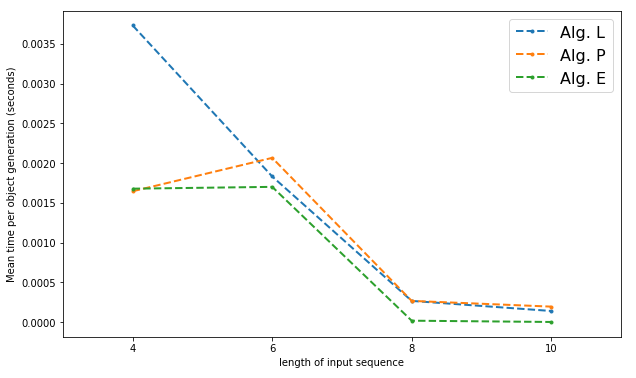
\includegraphics[width=0.8\textwidth]{images/perm_graph1.PNG}
\caption{Mean time to generate a permutation for some values of \(n\).}
\end{figure}

Algorithm E outperforms the other two for almost all values of \(n\) that were tested. Interestingly, the mean time decreases as \(n\) increases. This may appear counter-intuitive, given that the algorithms need to loop over a larger array. There are several reasons for this decrease. The overhead of initializing the arrays and variables at the start of the algorithm is distributed across all permutations, decreasing the average time. As \(n\) increases, the most common steps for generating the next object occur more and more often. Combine this with the increased efficiency of caching in memory when using lists in Python, this accounts for the overall decrease in the mean time.

Algorithm E was selected as the best performer based on the above results, and as such was implemented using \textit{Cython}. After calculating the mean times for both Algorithm E and \textit{itertools}, the following results were observed:

\begin{figure}[h]
\centering
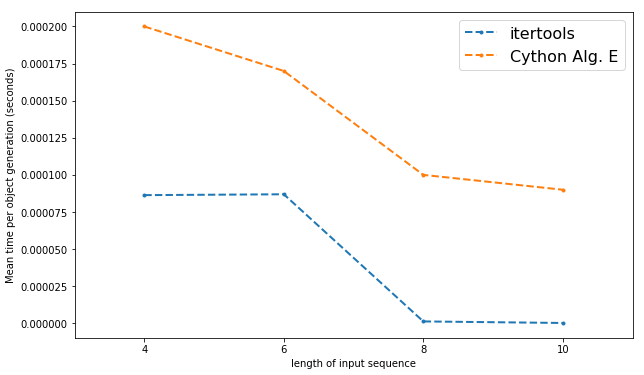
\includegraphics[width=0.8\textwidth]{images/perm_graph2.PNG}
\caption{Algorithm E in Cython vs \textit{itertools} for some values of \(n\).}
\end{figure}

\textit{Itertools} wins out against Algorithm E. We do see marked improvements in Algorithm E, however, compared to the default Python implementation. While Algorithm E was never going to match \textit{itertools} due to its implementation in pure C, it does offer a competitive and viable alternative.

For the random permutation algorithm \cite{rand_perm}, the following frequencies were observed for 100,000 iterations of the algorithm.

\begin{figure}[h]
\centering
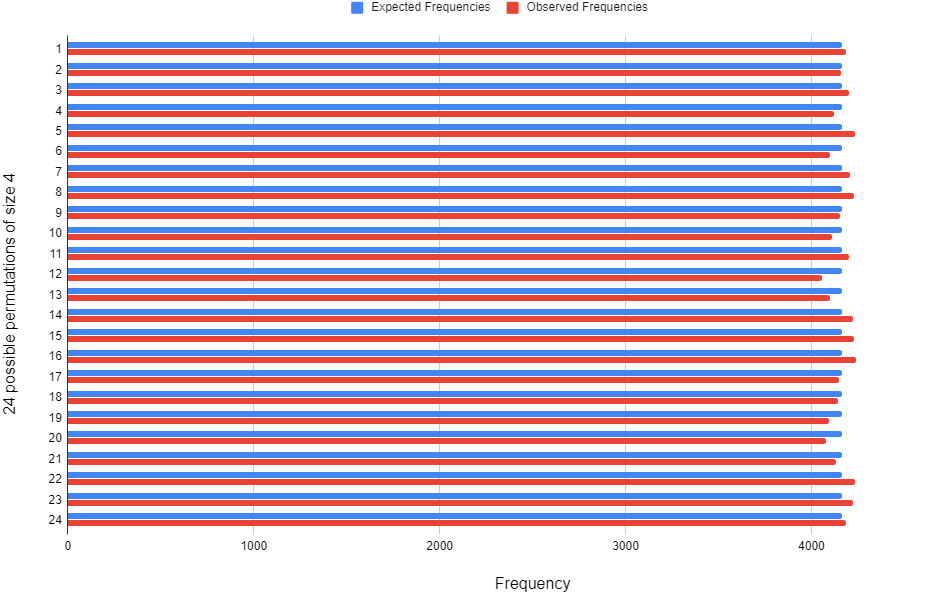
\includegraphics[width=1.0\textwidth]{images/perm_freq.PNG}
\caption{Expected vs Observed Frequencies}
\end{figure}

\pagebreak

The observed frequencies tend to close match the actual frequencies. Performing the chi-squared test on the observed frequencies returns \(p-value=0.64\). This is relatively high, and states that given a uniform distribution, the probability of seeing the observed frequencies is approximately \(64\%\). This is not enough to reject the null hypothesis, affirming the randomness of the algorithm.

\subsubsection{Combinations}
The same process used for permutations is repeated here. The size of the combinations being generated was locked to four, and the length of the sequences then vary to change the amount of combinations that are being generated.

\begin{figure}[h]
\centering
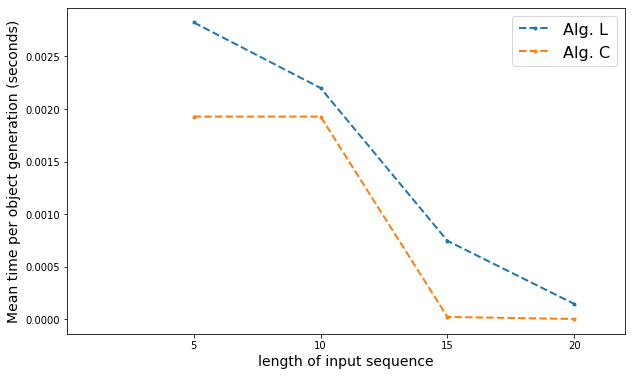
\includegraphics[width=1.0\textwidth]{images/comb_graph1.PNG}
\caption{Mean time to generate a combination for some values of \(n\)}
\end{figure}

\pagebreak

These algorithms follow a similar trend to the algorithms for permutations. Algorithm C boasts favourable results for all lengths of input sequences. The mean time decreases as \(n\) increases for the same reasons specified in the previous section. Algorithm C was enhanced with \textit{Cython} and compared to \textit{itertools}.

\begin{figure}[h]
\centering
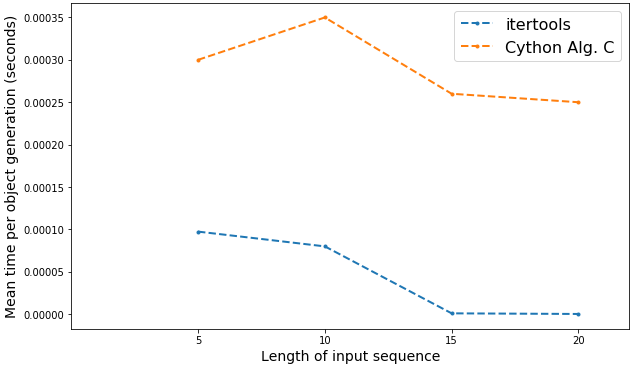
\includegraphics[width=1.0\textwidth]{images/comb_graph2.PNG}
\caption{Evaluation \textit{itertools} combination method to Algorithm C \cite{comb_C}}
\end{figure}

\pagebreak

The \textit{Cython} implementation of Algorithm C has a significant performance increase, but not enough to match \textit{itertools}. It is not quite as competitive as the package's permutation generator, but it generates combinations at a sufficient rate.

The frequencies were recorded for the 21 combinations of \(7 \choose 5\), as a similar amount of outcomes is favourable to keep the experiments fair and unbiased. Figure 23 illustrates a plausible random distribution of frequencies.

\begin{figure}[h]
\centering
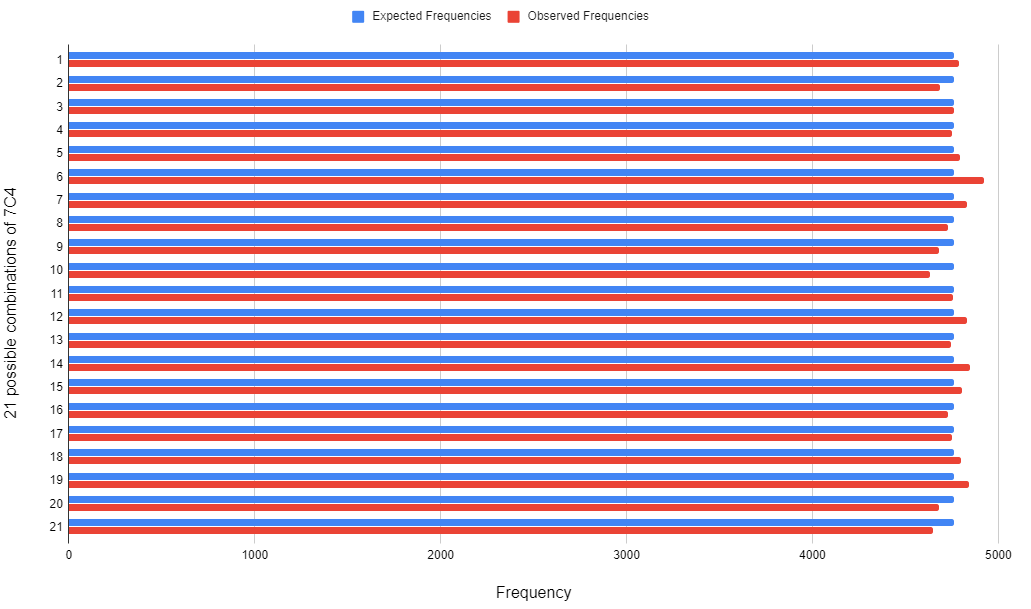
\includegraphics[width=1.0\textwidth]{images/comb_freq.PNG}
\caption{Frequency distribution of random combinations \cite{rand_comb}}
\end{figure}

The chi-squared test null hypothesis for this case states that the frequencies are independent, and maintain no relation to each other. The \(p-value=0.35\) was obtained by running the test on the observed combination frequencies. While lower than the \(p-value\) for permutations, it is still significantly higher than the required \(p-value=0.05\) to reject the null hypothesis. Thus, it can be said with some degree of certainty that this implementation produces suitably random results.

For the sake of completeness, the experiment was reran for \(7 \choose 3\). This was to verify the the improvement made by utilising an enhancement suggested by Knuth, discussed earlier in section 4.1.2 \cite{rand_comb}. That is to say, both selection sampling and rejection sampling produce random results. The \(p-value\) obtained was \(0.63\), which reiterates the assertion that the algorithm is random.

\subsubsection{Partitions}
Apart from testing the algorithms to verify that they produced all the correct outputs, there was little comparison to be done due to the lack of variety. One of the test that was carried out, was whether Algorithm H \cite{int_part_H} could produce the same outputs and Algorithm P \cite{int_part_P} when wrapped in a \lstinline{for} loop to specify the varying amount of partitions. 

\begin{figure}[h]
\centering
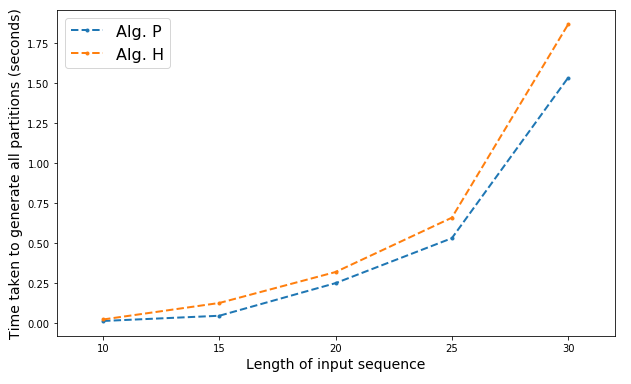
\includegraphics[width=1.0\textwidth]{images/int_part_graph.PNG}
\caption{A comparison between Algorithm P \cite{int_part_P} and Algorithm H \cite{int_part_H} for integer partitioning}
\end{figure}

The resulting graph nicely illustrates the exponential increase in the number of integer partitions, as the integer increases. It also exposes the efficiency of Algorithm P for generating all partitions of differing sizes.

Nijenhuis \& Herbert's algorithm for set partitioning \cite{rand_set_part} must have its randomness verified by the chi-squared test. The algorithm specifies the number of partitions that the sequence should be divided into, so the choice was made to generate all 3-partitions of a set containing ten elements, give 36 unique partitions.

\pagebreak

\begin{figure}[h]
\centering
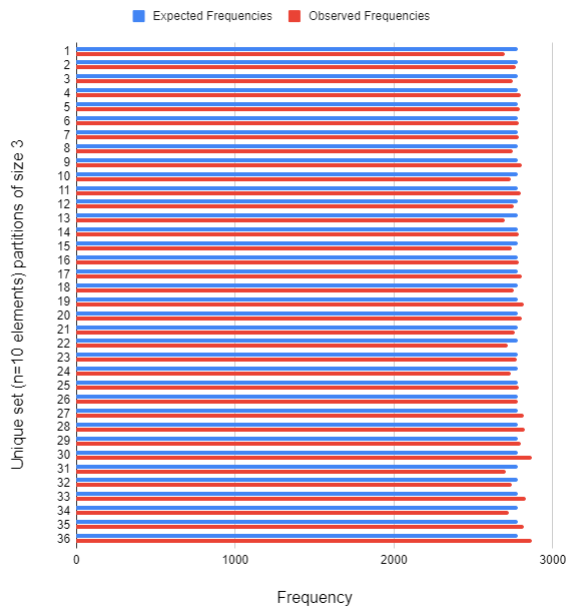
\includegraphics[width=0.8\textwidth]{images/set_part_freq.PNG}
\caption{The expected and observed frequencies of a random set partitioning algorithm \cite{rand_set_part}}
\end{figure}

The chi-squared test verified the functions randomness, returning \(p-value=0.93\). This overwhelmingly supports the null hypothesis, that there is no relationship between the set partitions.

\subsubsection{Trees}
Graphing the distribution of frequencies for Algorithm W \cite{tree_W} uncovered undesirable results.

\begin{figure}[h]
\centering
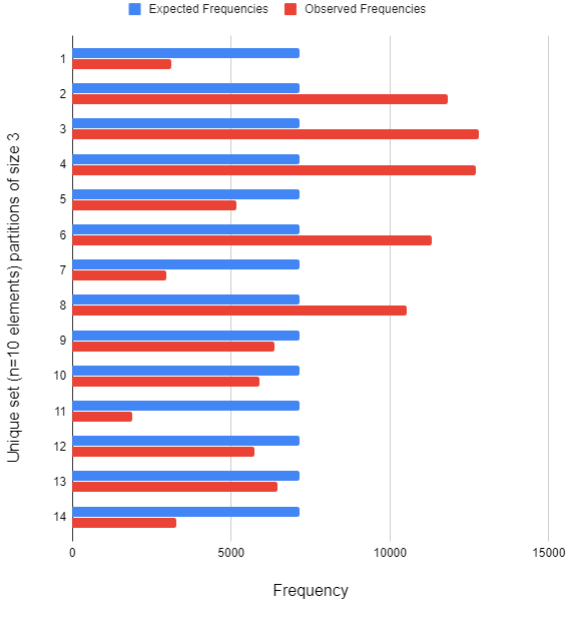
\includegraphics[width=0.8\textwidth]{images/rand_tree.PNG}
\caption{The expected and observed frequencies of a random tree generation algorithm}
\end{figure}

Visually, the distribution appears biased, with many observed frequencies that have tallies distant from the expected. This observation is supported by the chi-squared test, calculating \(p-value=0.0\), which unequivocally rejects the null hypothesis at a 5\% significance level. Evidently, Algorithm W does not generate uniformly random strings of nested parentheses, despite generating all of them at multiple times.

\pagebreak

% CONCLUSION ---------------------------------------------------------------------------------------------
\section{Conclusion}
The result of the project is a multipurpose package with the ability to generate the most common combinatorial objects. It enables developers to quickly access tools they need, instead of pulling resources from multiple different libraries. The project gives a voice to algorithms which otherwise may have been overlooked. Repeatedly, interesting and unexpected results cropped up. 

Knuth's algorithms performed comparably to \textit{itertools'} implementations of permutations and combinations. There is still room for improvement to be made here, which will explored in section 6.1. However, not all outcomes were as favourable as these, specifically Algorithm W for generating random trees. In spite of this hiccup, the other algorithms for generating random combinatorial objects all produced acceptably random results.

The work completed here is almost entirely based on existing knowledge. In \textit{The Art of Computer Programming Volume 1: Fundamental Algorithms}, Knuth says "an algorithm must be seen to be believed." This project supports his declaration, by giving a vision to algorithms, and providing competition to current standard. Competition is the greatest means of improvement and innovation.

\subsection{Future Work}
The area which immediately requires the most attention is the generation of random combinatorial objects. This package does not currently support such a method. The issue surely lies in the translation to Python, but it is not clear exactly where this occurs. On brief examination, the problem appears to lie with the source of entropy, and how the entropy is employed to attain uniform randomness. This is evident due to the correct objects appearing when the algorithm is employed sufficiently at least once. Additional work in this area should be focused on correcting what is a likely bug in the implementation, or researching new methods of random tree generation outside the scope of \textit{The Art of Computer Programming Volume 4A: Combinatorial Algorithms}.

Another area demanding attention is in the \textit{Cython} implementations of Algorithm E \cite{perm_E} and Algorithm C \cite{comb_C}. Rudimentary changes were made to the algorithms, offering significant improvement. The key to unlocking better performance lies in the use of data structures in the algorithms. Surprisingly, performance decreased after implementing C arrays instead of Python. As a result, these changes were withdrawn. The poor performance is likely due to the clumsy array manipulation in C, which led to shoddy loops over the arrays to change values. A promising solution to this employs \textit{numpy} arrays to act as the array structures. \textit{Numpy} allows  direct accessing of the data buffer at C speed, while maintaining better functionality supporting manipulation \cite{numpy}.

\subsection{How the Project was Conducted}
The project was divided into the four key problem areas: permutation, combinations, partitions, and trees. They were addressed one by one. The work started on permutations, in October 2019. Reading through Knuth's book was the initial step, where new concepts and ideas were introduced. Work began on implementing some of these algorithms in Python.

Come November 2019, the project moved on to look at combinations. The same approach was taken once again, and by the end of month, a package was beginning to take shape. There were now several algorithms which facilitated the generation of permutations and combinations. Work then slowed due to the looming exam season, before briefly continuing in late December and early January. Here, \textit{Cython} was explored. The package provided some competition to other packages.

Returning to college, the focus changes to trees. Growing more familiar with Knuth's work, the algorithms and ideas became easier to grasp. February saw partitions being explored, and by the end of the month, algorithms existed to offer functionality in each area. As the open-day approached, popular uses of the algorithms were investigated. This quickly ended however, due to the shutdown of the college. From here, work continued from home, attempting to shape the package further.

\subsection{Reflection}
The primary takeaway from this project is the effort required in order produce programming library of some substance. Before writing a single line of code, countless hours of research are needed in order to develop a satisfactory level of knowledge of an area. It is crucial to understand both theoretical and applied material that already exists in the problem space, to avoid repeating unnecessary work. Developing the project gave a fascinating insight into the tree-like structure that is the theoretical material. It was incredible to be able to trace ideas back through time, and relive the same realisations these great minds had before they wrote about them, all while nurturing an understanding of a momentous area of computer science.

% improved python
The process of developing the package promoted increased literacy in Python. Constant manipulation of lists in Python led to a greater understanding of the underlying data structures. Improvements were perpetually chased, aiding an ever-growing knowledge of the intricacies of Python.

% time management with virus
It would be unfair not to mention the global pandemic caused by the COVID-19 virus. Reflecting back on early March, there was no way to predict the disruption it would cause. Home suddenly became the only working environment available; not an ideal situation. In difficult and trying times, we turn to our friends and family for assistance. COVID-19 ripped this comfort away. 

The virus highlights the need for proper time-management. The future is unpredictable, and time is not a guarantee. Upon reflection, progress on this report should have began sooner. Although ideas and notes were kept from the beginning, the circumstances that arose have been detrimental. A more favourable approach would have been to start developing the report possibly as early as January, when the majority of the work on permutations and combinations was already complete. 

\pagebreak

\begin{thebibliography}{00}

\bibitem{chi_square}
Chi-squared statistical hypothesis test in \textit{SciPy} package for Python. URL: \url{https://docs.scipy.org/doc/scipy/reference/generated/scipy.stats.chisquare.html}

\bibitem{cython}
Cython static compiler for Python. URL: \url{https://cython.org/}

\bibitem{rand_perm}
Fisher, Ronald A.; Yates, Frank. \textit{Statistical tables for biological, agricultural and medical research (3rd ed.)} (1948) [1938], pp. 26–27

\bibitem{itertools}
\textit{itertools} Python package. URL: \url{https://docs.python.org/3/library/itertools.html}

\bibitem{itertools_extension}
\textit{itertools} Python package extension tools. \url{https://docs.python.org/3/library/itertools.html#itertools-recipes}

\bibitem{rand_comb}
Knuth, Donald. The Art of Computer Programming Volume 2, \textit{Seminumerical Algorithms} 3.4.2 (1998), pp. 142-143.

\bibitem{knuth_shuffle}
Knuth, Donald. The Art of Computer Programming Volume 2, \textit{Seminumerical Algorithms} 3.4.2 (1998), pp. 145.

\bibitem{perm_L}
Knuth, Donald. The Art of Computer Programming Volume 4, \textit{Combinatorial Algorithms} 7.2.1.2 (2005), pp. 1-2. URL: \url{http://www.cs.utsa.edu/~wagner/knuth/fasc2b.pdf}

\bibitem{perm_P}
Knuth, Donald. The Art of Computer Programming Volume 4, \textit{Combinatorial Algorithms} 7.2.1.2 (2005), pp. 4. URL: \url{http://www.cs.utsa.edu/~wagner/knuth/fasc2b.pdf}

\bibitem{perm_E}
Knuth, Donald. The Art of Computer Programming Volume 4, \textit{Combinatorial Algorithms} 7.2.1.2 (2005), pp. 19-20. URL: \url{http://www.cs.utsa.edu/~wagner/knuth/fasc2b.pdf}

\bibitem{perm_G}
Knuth, Donald. The Art of Computer Programming Volume 4, \textit{Combinatorial Algorithms} 7.2.1.2 (2005), pp. 11. URL: \url{http://www.cs.utsa.edu/~wagner/knuth/fasc2b.pdf}

\bibitem{comb_L}
Knuth, Donald. The Art of Computer Programming Volume 4, \textit{Combinatorial Algorithms} 7.2.1.3 (2005), pp. 4-5. URL: \url{http://www.cs.utsa.edu/~wagner/knuth/fasc3a.pdf}

\bibitem{comb_T}
Knuth, Donald. The Art of Computer Programming Volume 4, \textit{Combinatorial Algorithms} 7.2.1.3 (2005), pp. 5. URL: \url{http://www.cs.utsa.edu/~wagner/knuth/fasc3a.pdf}

\bibitem{comb_C}
Knuth, Donald. The Art of Computer Programming Volume 4, \textit{Combinatorial Algorithms} 7.2.1.3 (2005), pp. 11-15. URL: \url{http://www.cs.utsa.edu/~wagner/knuth/fasc3a.pdf}

\bibitem{int_part_P}
Knuth, Donald. The Art of Computer Programming Volume 4, \textit{Combinatorial Algorithms} 7.2.1.4 (2005), pp. 2. URL: \url{http://www.cs.utsa.edu/~wagner/knuth/fasc3b.pdf}

\bibitem{int_part_H}
Knuth, Donald. The Art of Computer Programming Volume 4, \textit{Combinatorial Algorithms} 7.2.1.4 (2005), pp. 2-3. URL: \url{http://www.cs.utsa.edu/~wagner/knuth/fasc3b.pdf}

\bibitem{set_part_H}
Knuth, Donald. The Art of Computer Programming Volume 4, \textit{Combinatorial Algorithms} 7.2.1.5 (2005), pp. 26-27. URL: \url{http://www.cs.utsa.edu/~wagner/knuth/fasc3b.pdf}

\bibitem{tree_P}
Knuth, Donald. The Art of Computer Programming Volume 4, \textit{Combinatorial Algorithms} 7.2.1.6 (2005), pp. 2-3. URL: \url{http://www.cs.utsa.edu/~wagner/knuth/fasc4a.pdf}

\bibitem{tree_B}
Knuth, Donald. The Art of Computer Programming Volume 4, \textit{Combinatorial Algorithms} 7.2.1.6 (2005), pp. 4-5. URL: \url{http://www.cs.utsa.edu/~wagner/knuth/fasc4a.pdf}

\bibitem{tree_W}
Knuth, Donald. The Art of Computer Programming Volume 4, \textit{Combinatorial Algorithms} 7.2.1.6 (2005), pp. 13. URL: \url{http://www.cs.utsa.edu/~wagner/knuth/fasc4a.pdf}

\bibitem{rand_set_part}
Nijenhuis, Albert; Herbert, Wilf. \textit{Combinatorial Algorithms For Computers and Calculators 2nd Edition} (1978), pp. 52-53. URL: \url{https://www.math.upenn.edu/~wilf/website/CombinatorialAlgorithms.pdf}

\bibitem{numpy}
\textit{NumPy} Python package. URL: \url{https://cython.readthedocs.io/en/latest/src/userguide/numpy_tutorial.html#efficient-indexing-with-memoryviews}

\bibitem{generator}
Python Generator Functions. URL: \url{https://wiki.python.org/moin/Generators}

\end{thebibliography}

\end{document}
